% preamble with all definitions
\documentclass[12pt,letterpaper]{article}
\usepackage[utf8]{inputenc}
\usepackage[english]{babel}
\usepackage{amsmath}
\usepackage{amsfonts}
\usepackage{amssymb}
\usepackage{graphicx}
\usepackage{multirow}
\usepackage{fancyvrb}
\usepackage[breaklinks=true]{hyperref}
\usepackage[hyphenbreaks]{breakurl}
\hypersetup{
       pdfauthor = {Kim Siang Khaw},
        colorlinks=true, citecolor=blue, linkcolor=blue, bookmarksnumbered = true,
}
\usepackage[left=2cm,right=2cm,top=2cm,bottom=2cm]{geometry}

%%%%%%%Some style changes
\usepackage{caption}
\setlength{\captionmargin}{10mm}
\renewcommand\captionfont{\it}
\renewcommand\captionlabelfont{\bf}


\author{Wes Gohn, Tim Gorringe, Ran Hong, Kim Siang Khaw, David Sweigart}
\title{\textbf{DAQ data structure for the Muon g-2 experiment}}
\begin{document}

\maketitle

\abstract{
This document outlines the DAQ data structure of the Muon g-2 experiment.
A detailed list of the MIDAS data bank will be shown and their contents will 
described.}

\tableofcontents
\newpage

\section{MIDAS DAQ output in a nutshell}
The main DAQ framework for the Muon g-2 experiment is based on MIDAS [cite]. 
MIDAS event structure is as depicted in Fig.~\ref{fig:MIDASEventStructure}.

\begin{figure}[htbp]
\centering
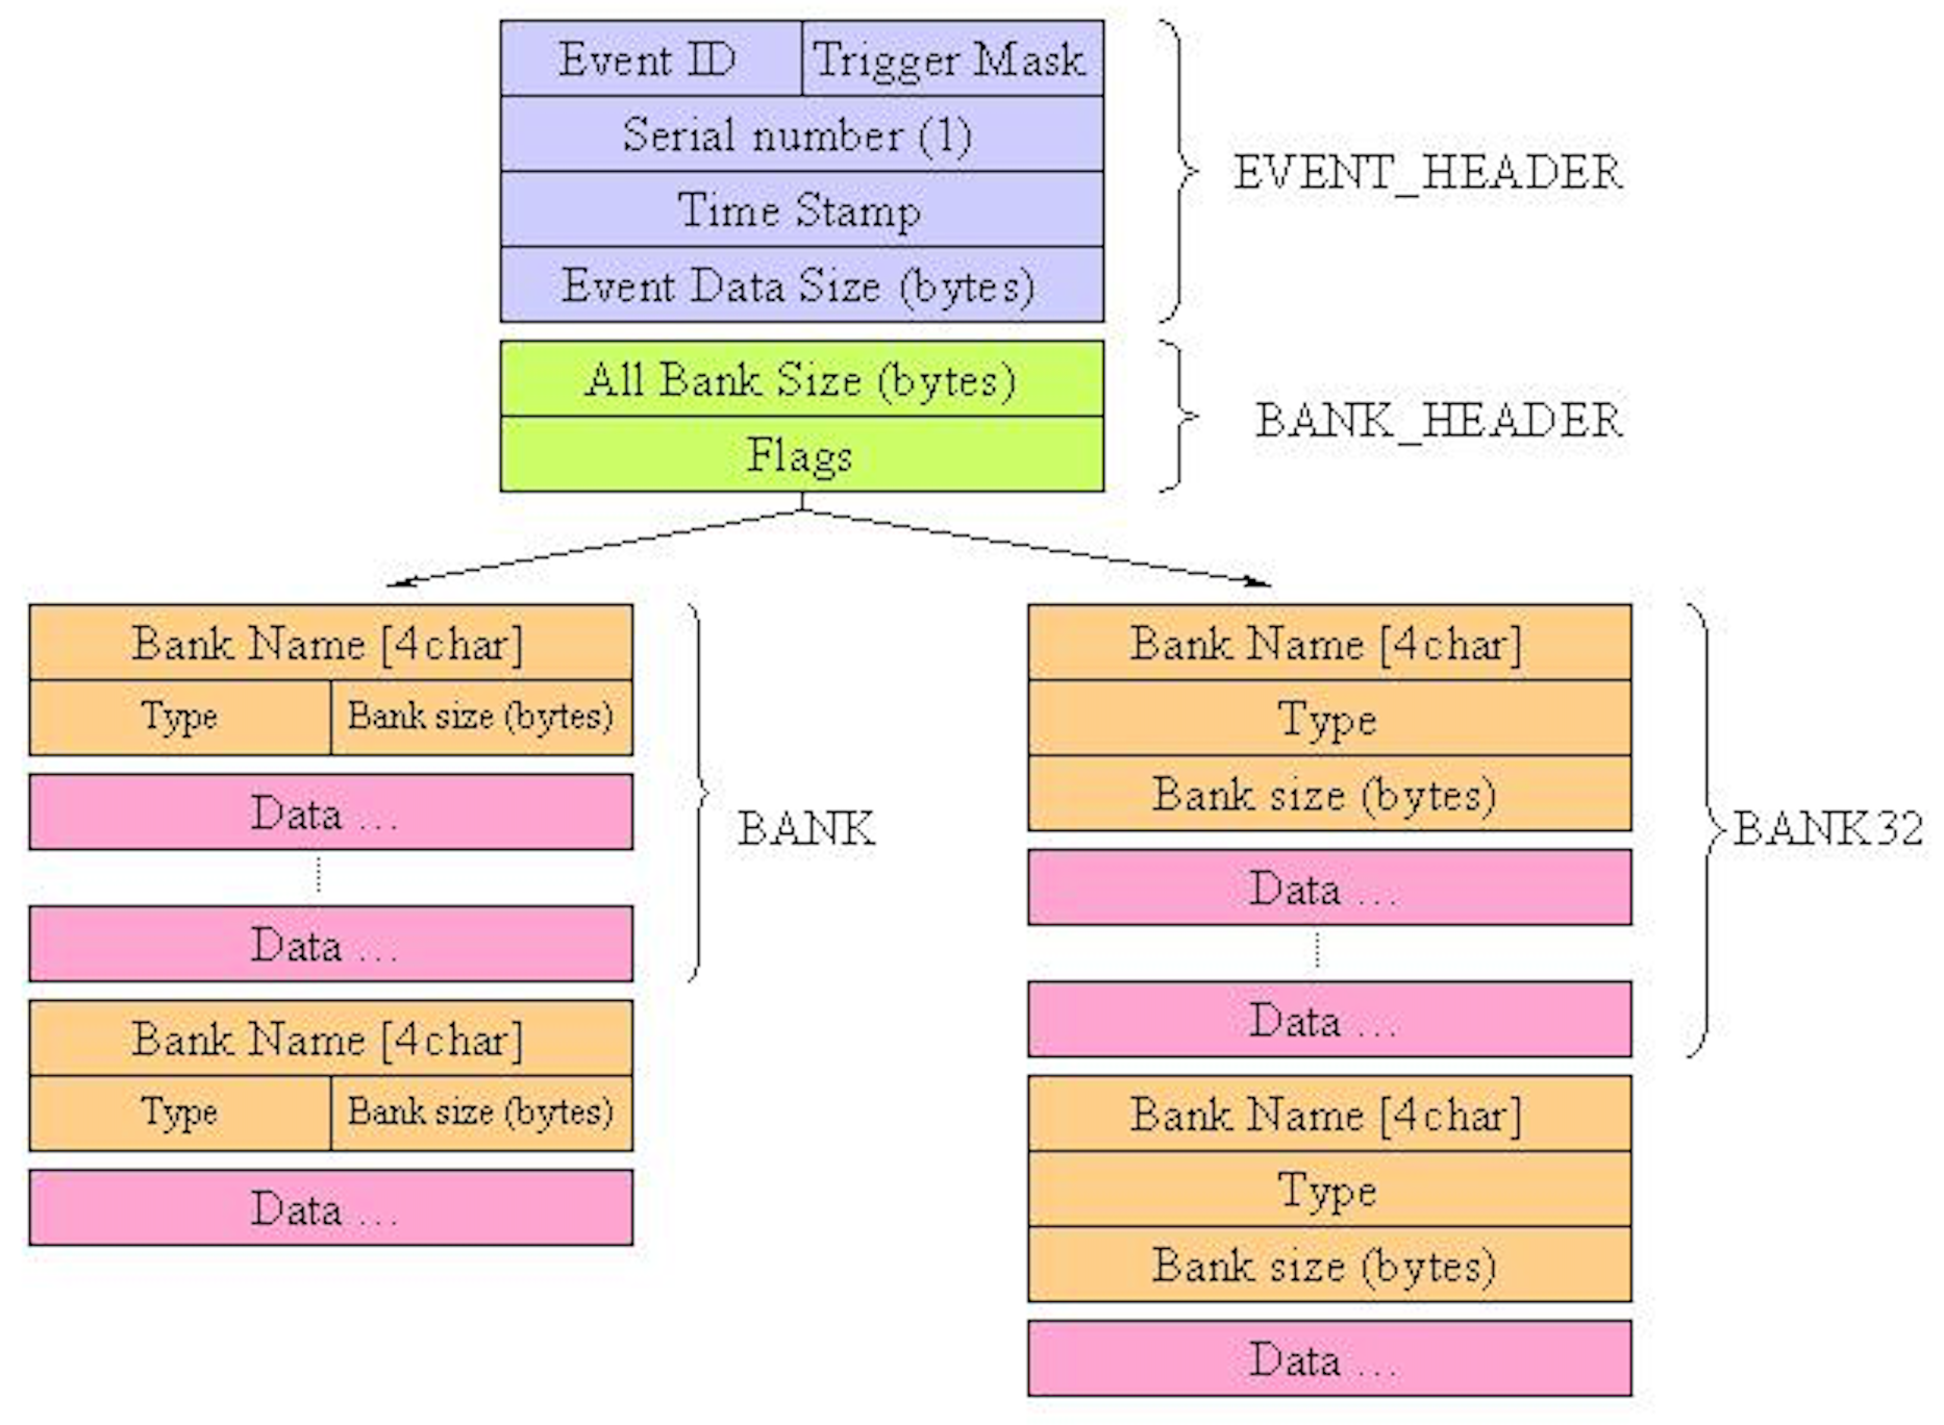
\includegraphics[width=0.6\textwidth]{pics/MIDASEventStructure.pdf} 
\caption{MIDAS event structure. Each event has its header that is followed by the bank header. Then all the banks will appear according the defined order.}\label{fig:MIDASEventStructure}
\end{figure}


\section{MIDAS Bank list}

Hundred of banks will be stored in each MIDAS event and it is very important to classify them properly. At the moment they can be grouped into 4 categories: calorimeter, auxiliary detector, CCC and magnetic field. Naming of these banks will be described in this section and their contents will be explained in the next section.

\subsection{Calorimeter-related banks}

There are 3 fill types for the calorimeter. \verb+Muon+ fill is the typical muon events, laser fill is event dedicated for laser calibration and monitoring events and pedestal fill is trivia from its name. Data from each fill type is identified from the bank name. The muon fill is denoted by ``\textbf{C}", the laser fill is denoted by ``\textbf{L}" and the pedestal fill is denoted by ``\textbf{P}". A summary of the banks is listed in Tab. \ref{tab:calotable}.

\begin{table}[htbp]
\centering
\caption{MIDAS bank list for the calorimetry data.}
\begin{tabular}{|c|c|c|c|}
\hline 
muon fill& laser fill & pedestal fill  & \multirow{2}{*}{Description} \\ \cline{1-3}
\multicolumn{3}{|c|}{Bank name} & \\
\hline
CA & LA & PA & AMC13 Header \\ 
\hline 
CB & LB & PB & WFD5 header \\ 
\hline 
CC & LC & PC & GPU timing data \\ 
\hline 
CF & LF & PF & GPU fitted data \\ 
\hline 
CH & LH & PH & per-crystal Q-method data (N-th event, end of run) \\ 
\hline 
CL & LL & PL & Clock data \\ 
\hline 
CP & LP & PP & Pedestal\\ 
\hline 
CQ & LQ & PQ & per-calo Q-method data (every event) \\ 
\hline 
CR & LR & PR & WFD5 raw data \\ 
\hline 
CT & LT & PT & T-method islands \\ 
\hline 
CZ & LZ & PZ & AMC13 CDF trailers \\ 
\hline 
\end{tabular} 
\label{tab:calotable}
\end{table}

\subsection{Auxiliary detector-related banks}

A separate T/Q-method is needed for auxiliary detectors. Their data banks are denoted with the initial ``\textbf{K}".
A list of these banks are summarized in Tab. \ref{tab:auxtable}.

\begin{table}[htbp]
\centering
\caption{MIDAS bank list for auxiliary T/Q data. This is mainly for the fiber harps, quads and kickers.}
\begin{tabular}{|c|c|}
\hline 
Bank name  & Description \\
\hline
KH &  Per aux. detector channel Q-method data (N-th event, end of run)\\
\hline
KQ &  Per aux. detector Q-method data (every event)\\
\hline
KT & T-method data \\
\hline
\end{tabular} 
\label{tab:auxtable}
\end{table}

\subsection{CCC related banks}

This is the bank housing information regarding the CCC system based on FC7.
A list of these banks are summarized in Tab. \ref{tab:ccctable}.

\begin{table}[htbp]
\centering
\caption{MIDAS bank list for the CCC data.}
\begin{tabular}{|c|c|}
\hline 
TTCA & AMC13 Header \\
\hline
TTCR & CCC AMC13 Payload\\
\hline
TTCZ & AMC13 Trailer \\
\hline
\end{tabular} 
\label{tab:ccctable}
\end{table}


\subsection{Field related banks}

Overall instructions: \\

All field-team banks are filled once per event.
For many field-team banks, a c struct is defined in the \verb+field_struct.hh+ file, accessible for all frontends and unpackers. Programmers should able to cast the read-out bank (array of bytes) onto a pointer of the corresponding struct. A midas bank can be an entire struct (like \textbf{TLNP}, \textbf{ABPR}, etc) or a array of structs (like \textbf{GALI}). A list of these banks are summarized in Tab. \ref{tab:fieldtable}.


\begin{table}[htbp]
\centering
\caption{MIDAS bank list for the magnetic field related data.}
\begin{tabular}{|c|c|p{11cm}|}
\hline
System & Name & Description \\
\hline
Fixed probe & FXPR & Fixed probe, header + NMR waveforms \\
\hline
\multirow{4}{*}{Trolley} & TLNP & Trolley NMR Pulse, header + NMR waveforms\\
\cline{2-3}
& TLBC &  Trolley Barcode, header + Barcode waveforms \\
\cline{2-3}
& TLMN & Trolley Monitors (temperatures, voltages and pressure), header + voltage waveforms \\
\cline{2-3}
& GALI &  Galil (trolley and garage) data, positions + velocities + control voltages + tensions\\
\hline
Absolute probes &  ABPR &
Absolute probe (spherical probe and plunging probe are using the same bank), header + NMR waveforms \\ 
\hline
Flux gate & FLUX & Flux gate, fluxgate waveforms \\
\hline
Surface coil & SFCL & Surface coil, current readouts\\
\hline
\end{tabular} 
\label{tab:fieldtable}
\end{table}

\section{Bank contents}

This section details contents of each MIDAS bank. 

\subsection{Calorimeter-related banks}

\subsubsection*{CA (LA, PA) and CZ (LZ, PZ) banks}

\begin{figure}[htbp]
\centering
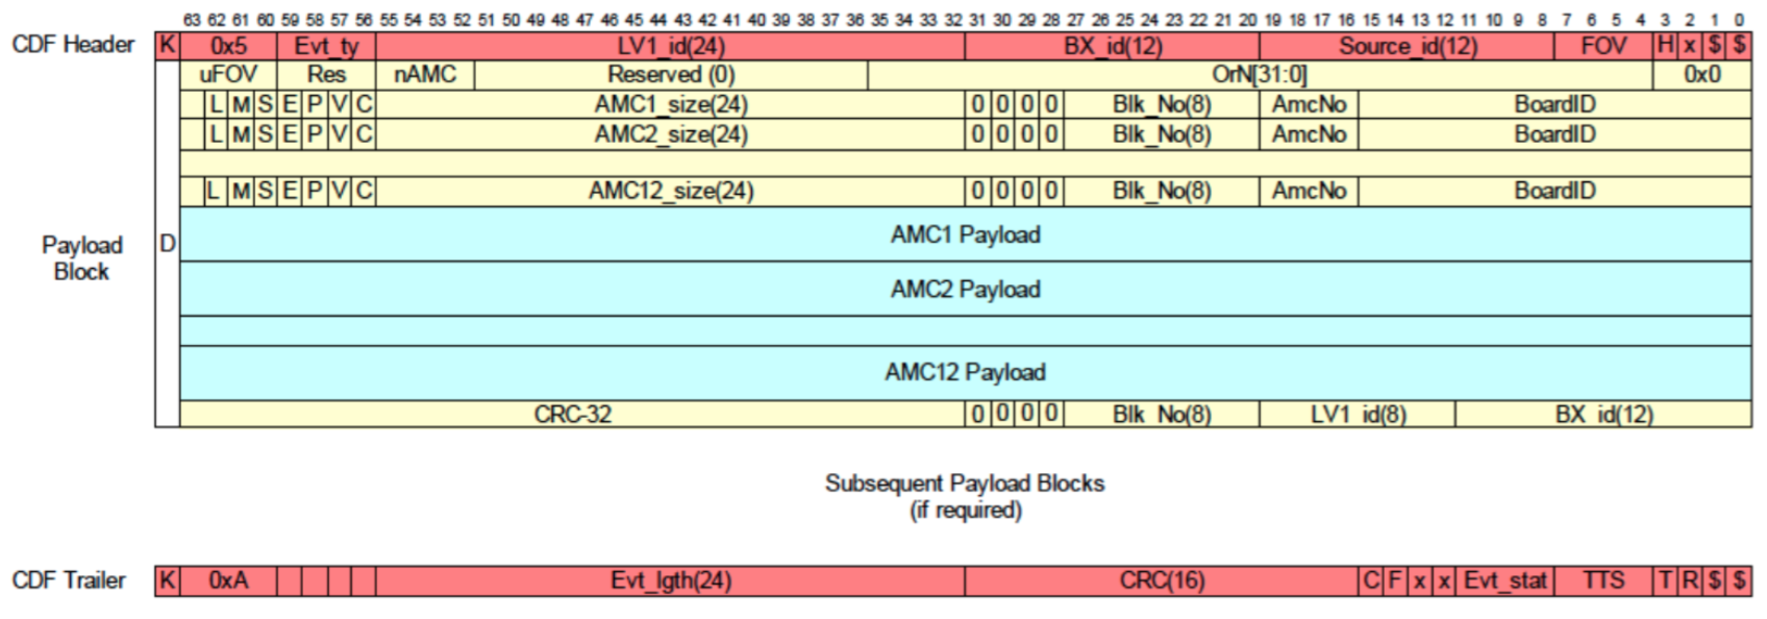
\includegraphics[width=0.85\textwidth]{pics/AMC13ToDAQ.pdf} 
\caption{Data structure for AMC13 to DAQ. The first 2 64-bit words are stored in the CA (LA, PA) bank.}\label{fig:AMC13ToDAQ}
\end{figure}

\subsubsection*{CB (LB, PB) banks}

\begin{figure}[htbp]
\centering
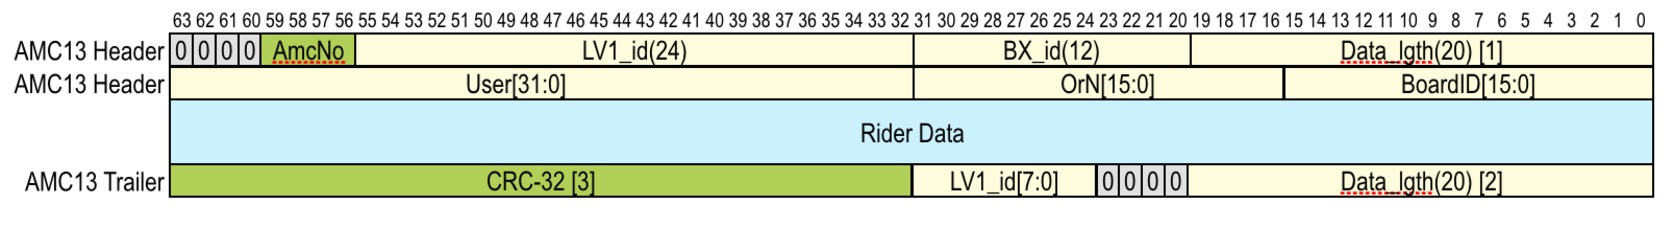
\includegraphics[width=0.85\textwidth]{pics/RiderToAMC13.pdf} 
\caption{Data structure for Rider to AMC13.}\label{fig:RiderToAMC13}
\end{figure}

\subsubsection*{CR (LR, PR) banks}

This is the bank for the full WFD5 payload.

\begin{figure}[htbp]
\centering
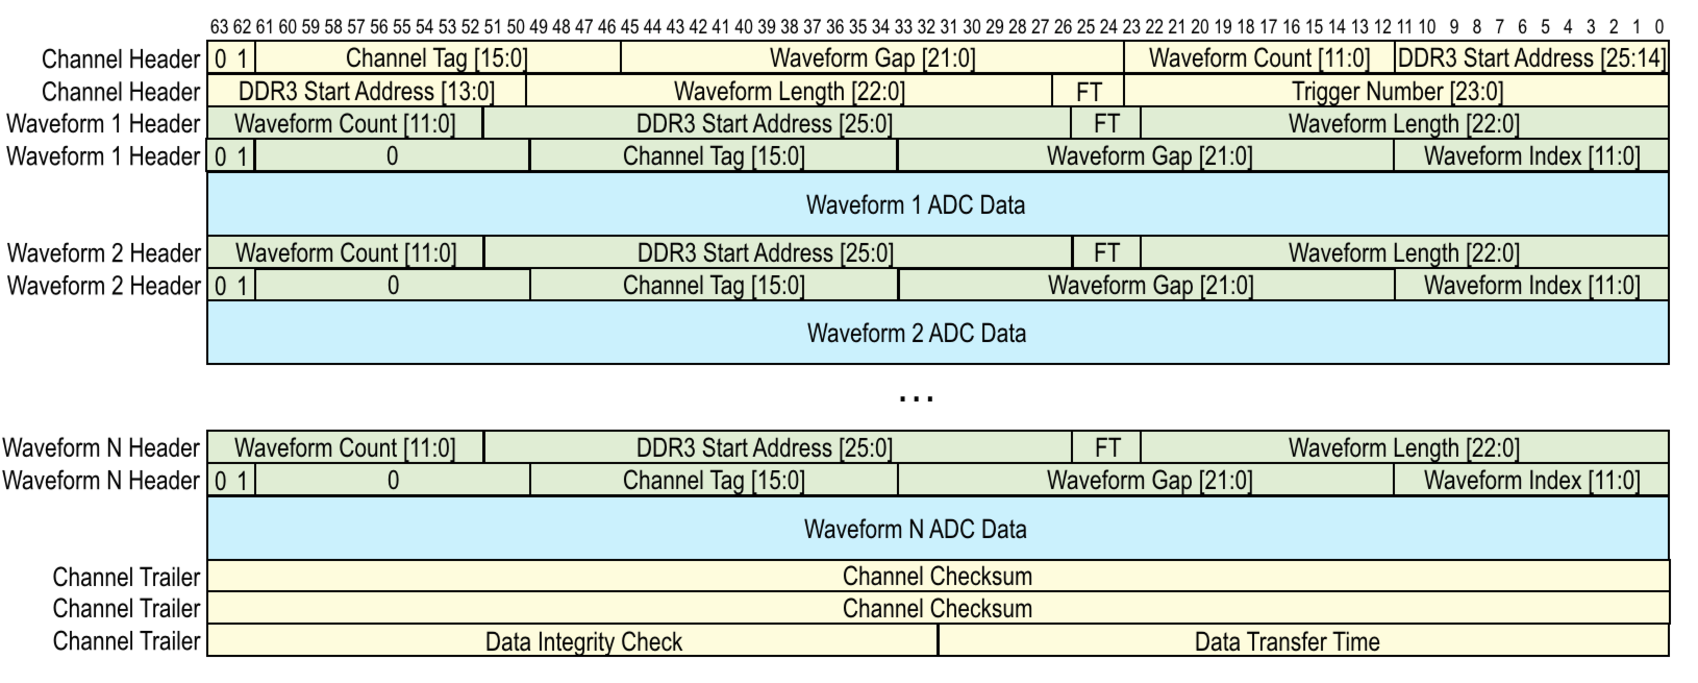
\includegraphics[width=0.85\textwidth]{pics/RiderData.pdf} 
\caption{Data structure for the WFD5 raw payload.}\label{fig:RiderData}
\end{figure}

\subsubsection*{C? (L?, P?) banks, TBD}

This is the bank for the WFD5 payload in the asynchronous mode.

\begin{figure}[htbp]
\centering
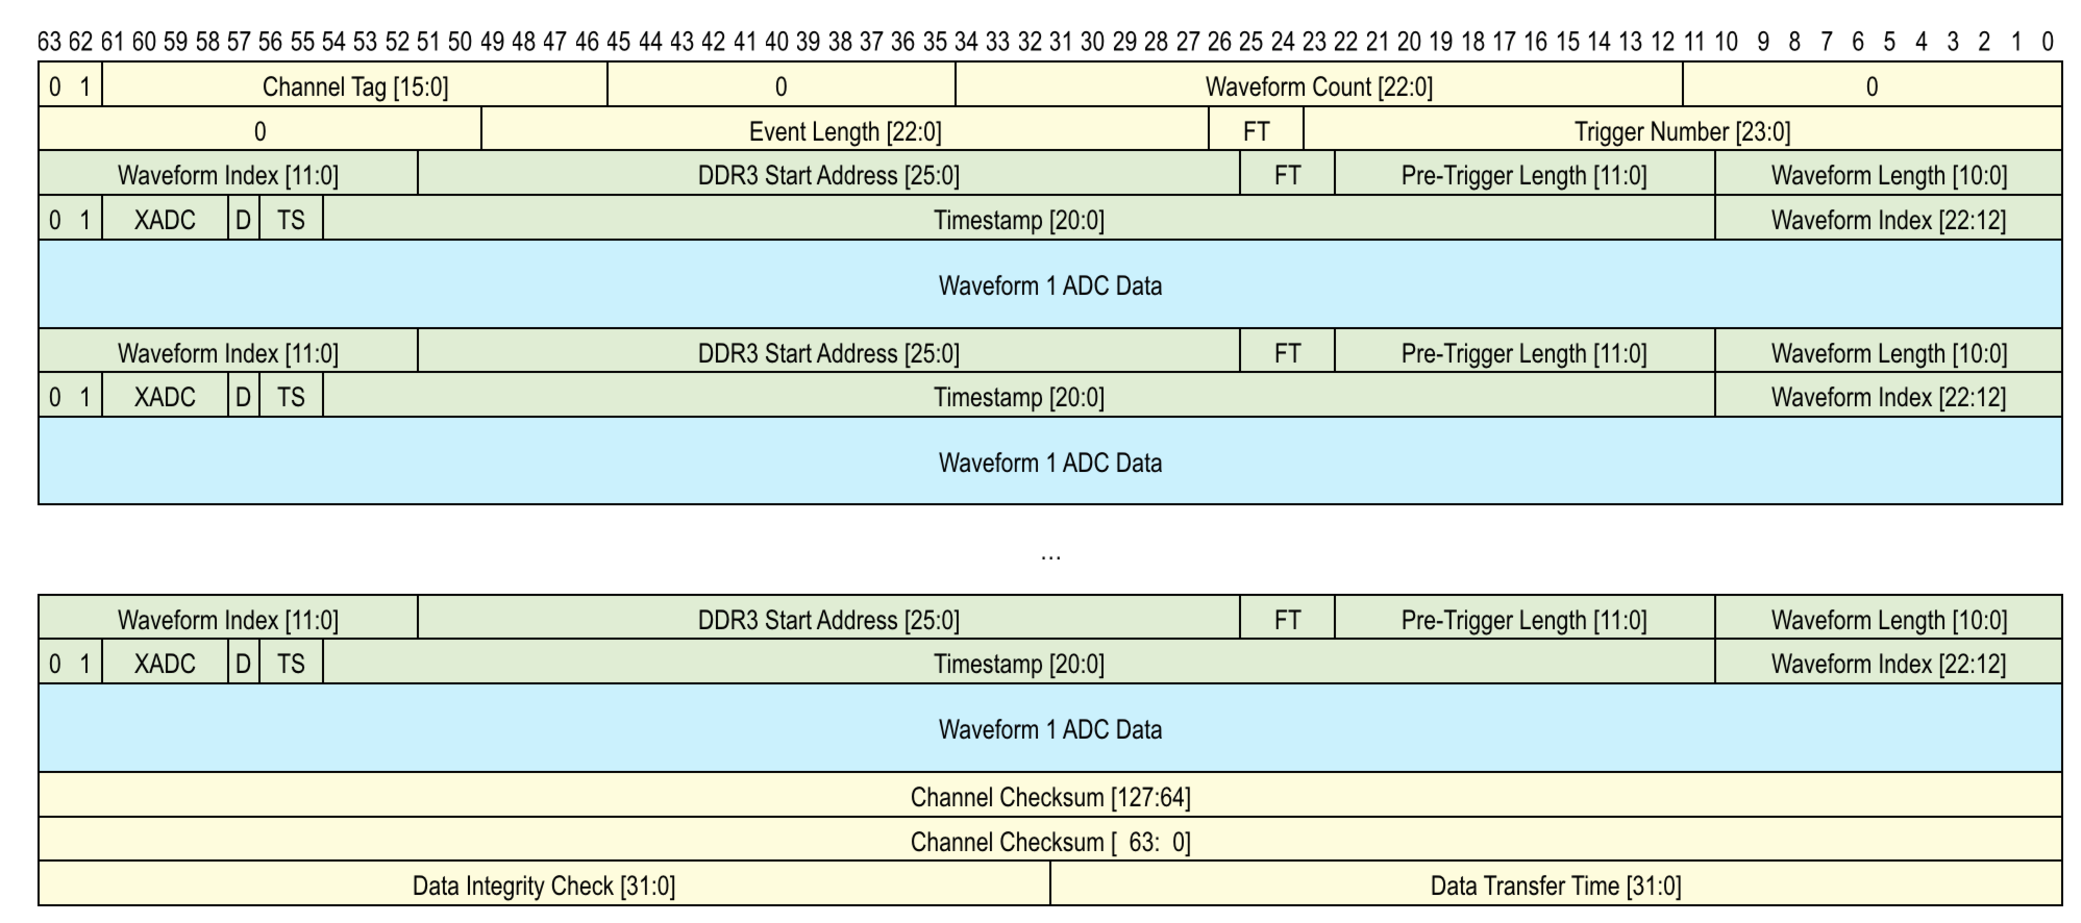
\includegraphics[width=0.85\textwidth]{pics/AsyncRiderData.pdf} 
\caption{Data structure for asynchronous mode for Rider.}\label{fig:AsyncRiderData}
\end{figure}


\subsubsection*{CT (LT, PT) banks}

\begin{figure}[htbp]
\centering
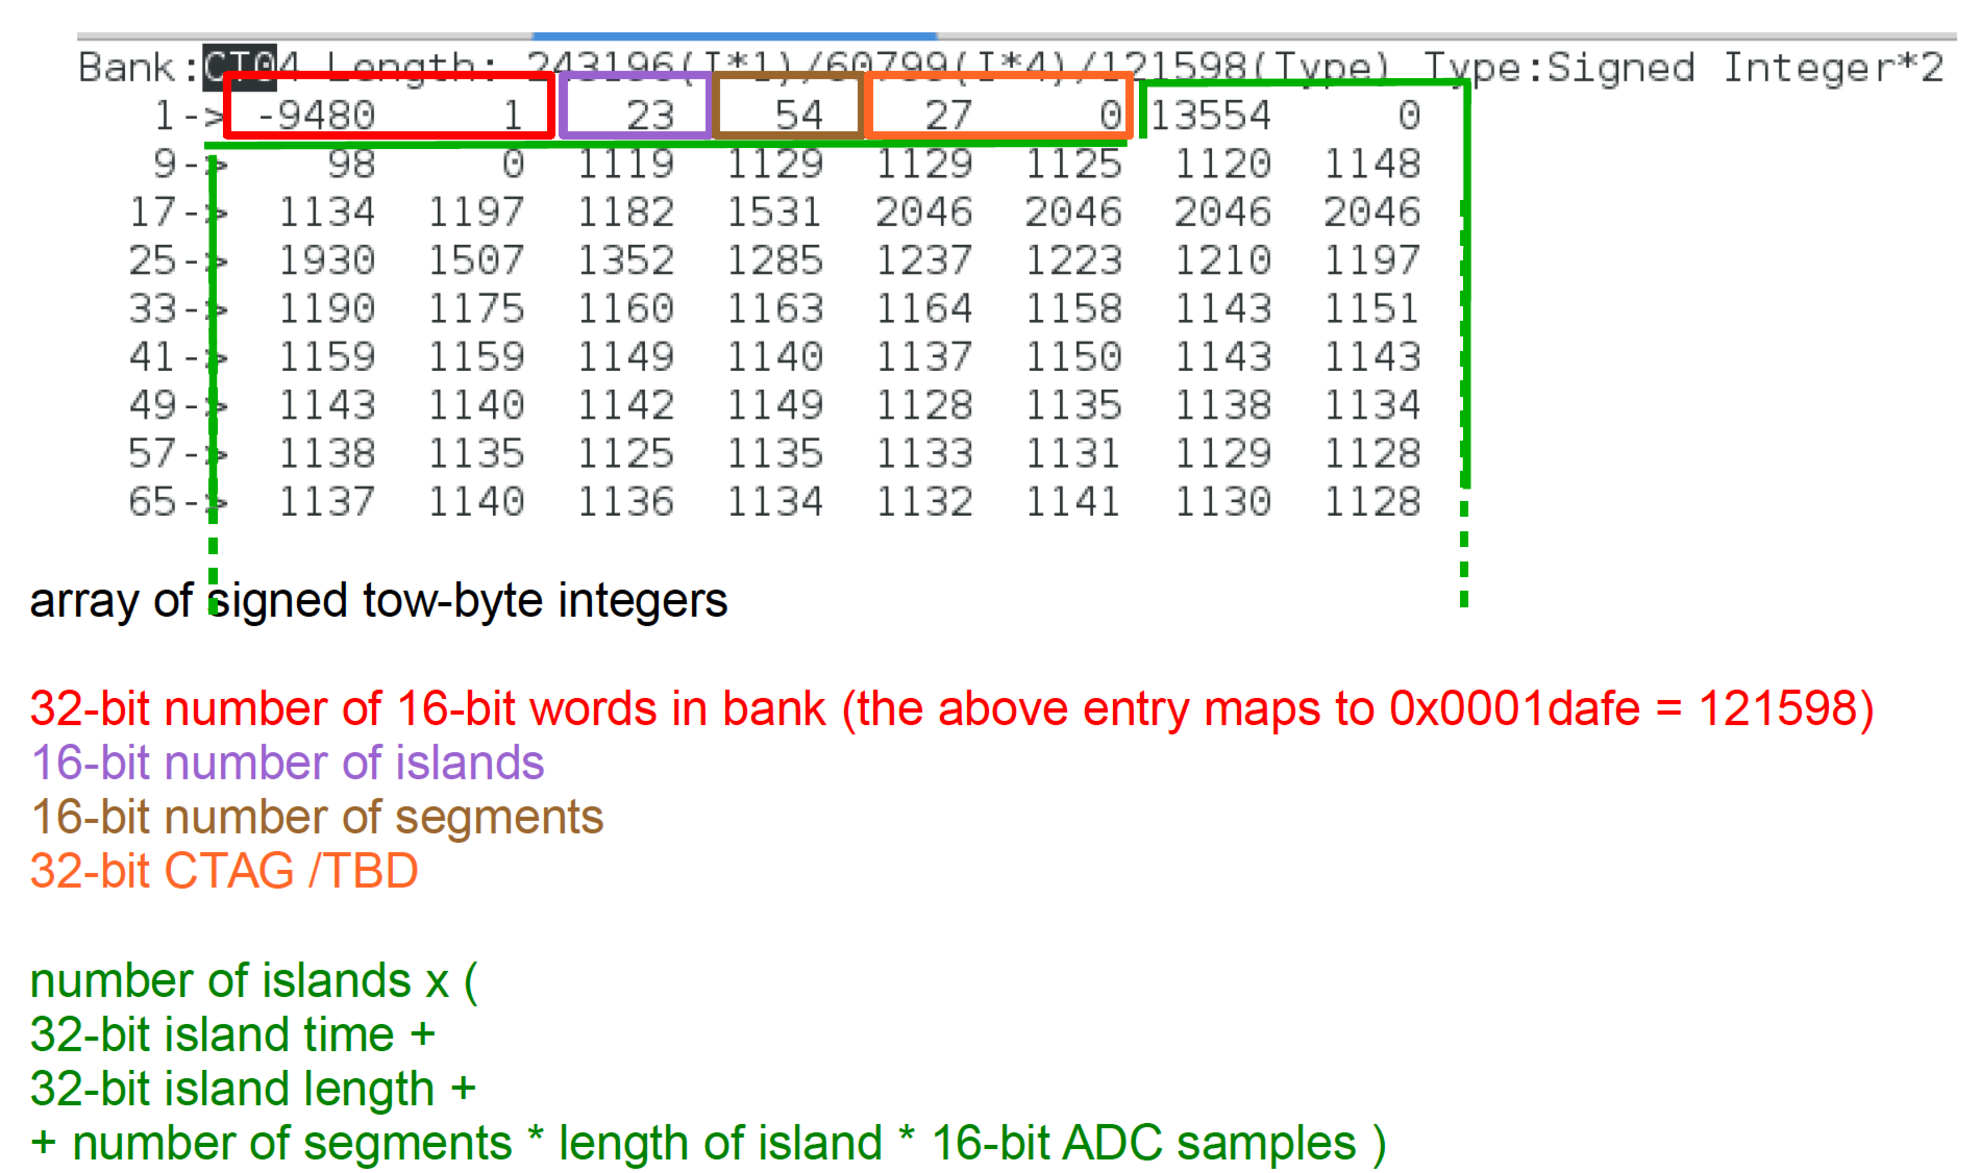
\includegraphics[width=0.85\textwidth]{pics/CTBankFormat.pdf} 
\caption{Data structure for the CT bank (T-method chopped islands).}\label{fig:CTBankFormat}
\end{figure}

\subsubsection*{CH (LH, PH) banks}

\begin{figure}[htbp]
\centering
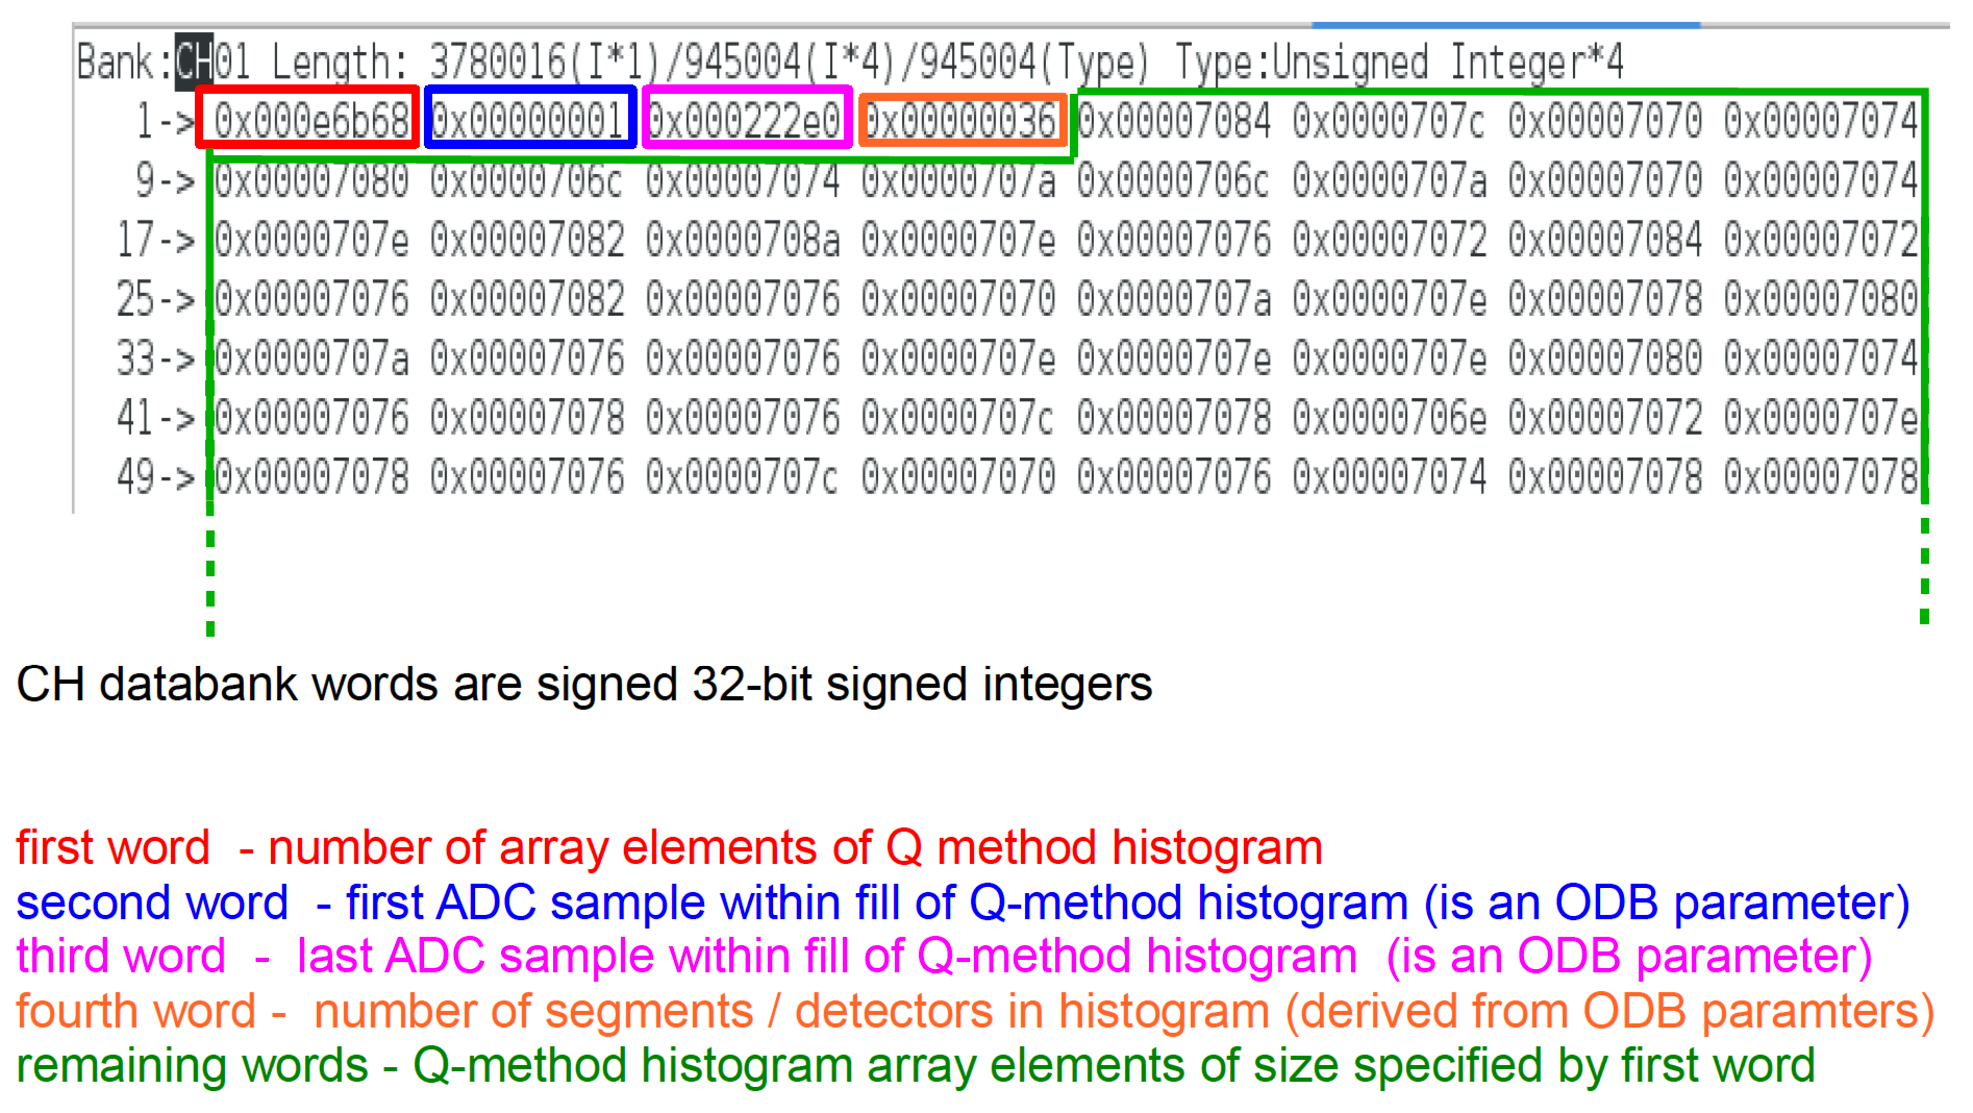
\includegraphics[width=0.85\textwidth]{pics/CHBankFormat.pdf} 
\caption{Data structure for the CH bank (calo segment histograms).}\label{fig:CHBankFormat}
\end{figure}

\subsubsection*{CQ (LQ, PQ) banks}

\begin{figure}[htbp]
\centering
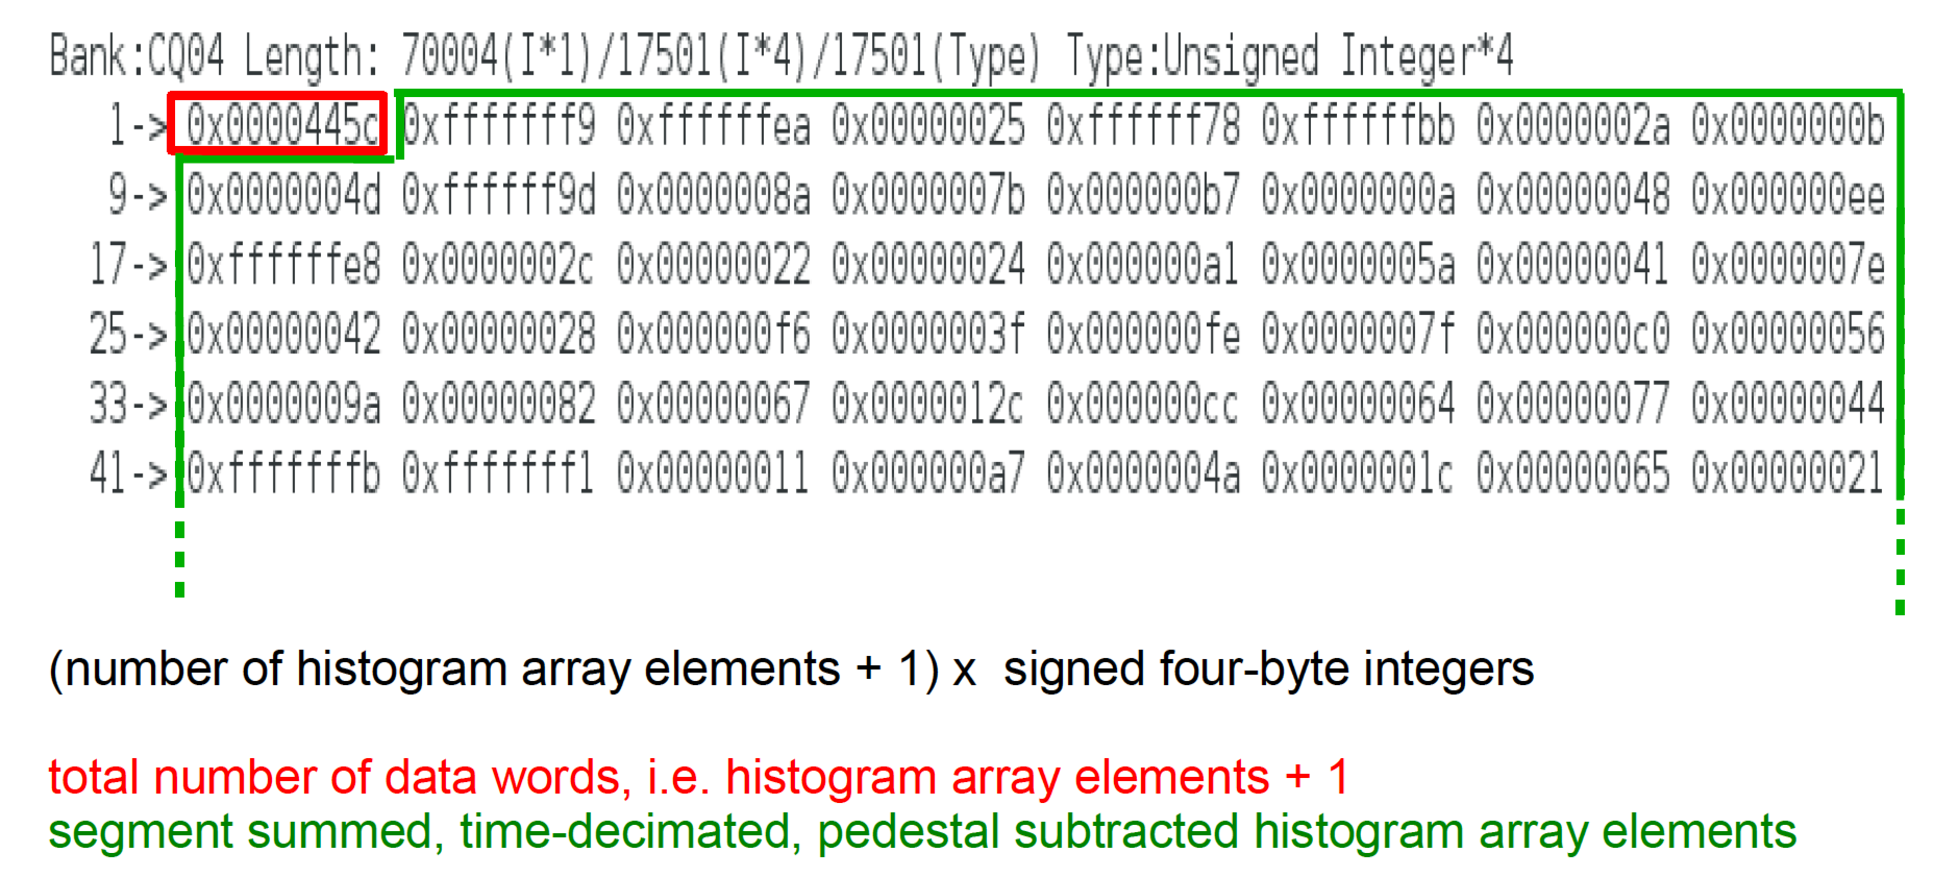
\includegraphics[width=0.85\textwidth]{pics/CQBankFormat.pdf} 
\caption{Data structure for the CQ bank (calo sum histograms).}\label{fig:CQBankFormat}
\end{figure}

\subsubsection*{CP (LP, PP) banks}

\begin{figure}[htbp]
\centering
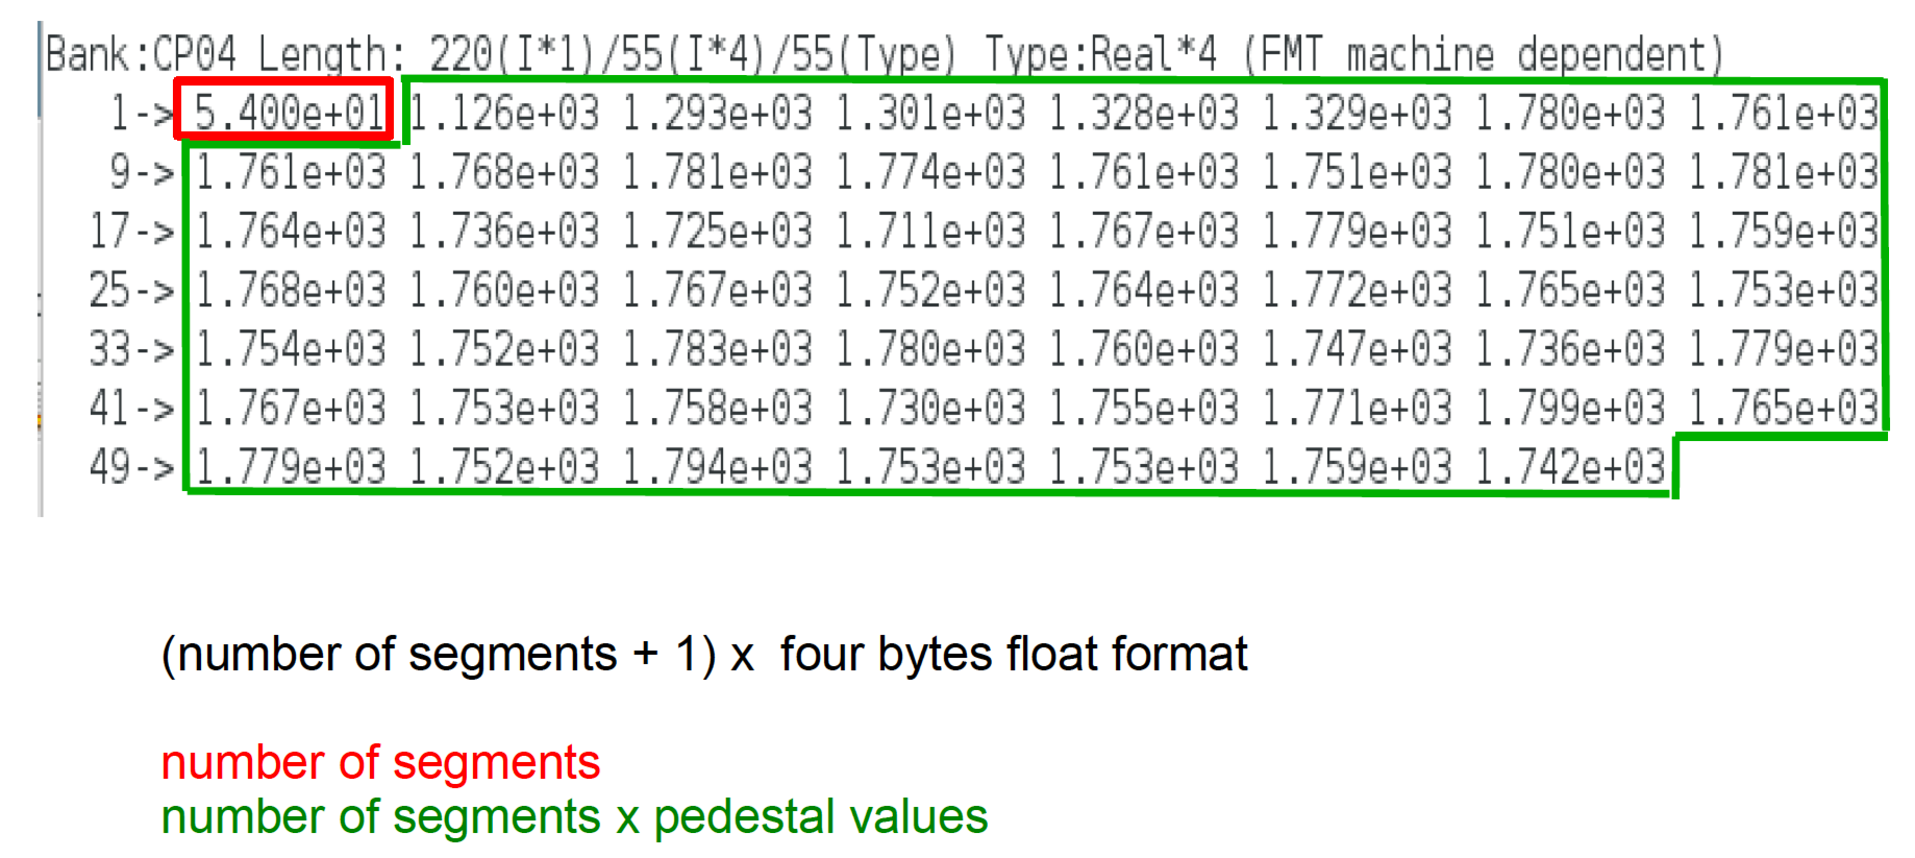
\includegraphics[width=0.85\textwidth]{pics/CPBankFormat.pdf} 
\caption{Data structure for the CP bank (T-method pedestals).}\label{fig:CPBankFormat}
\end{figure}

\subsubsection*{CC (LC, PC) banks}


\begin{figure}[htbp]
\centering
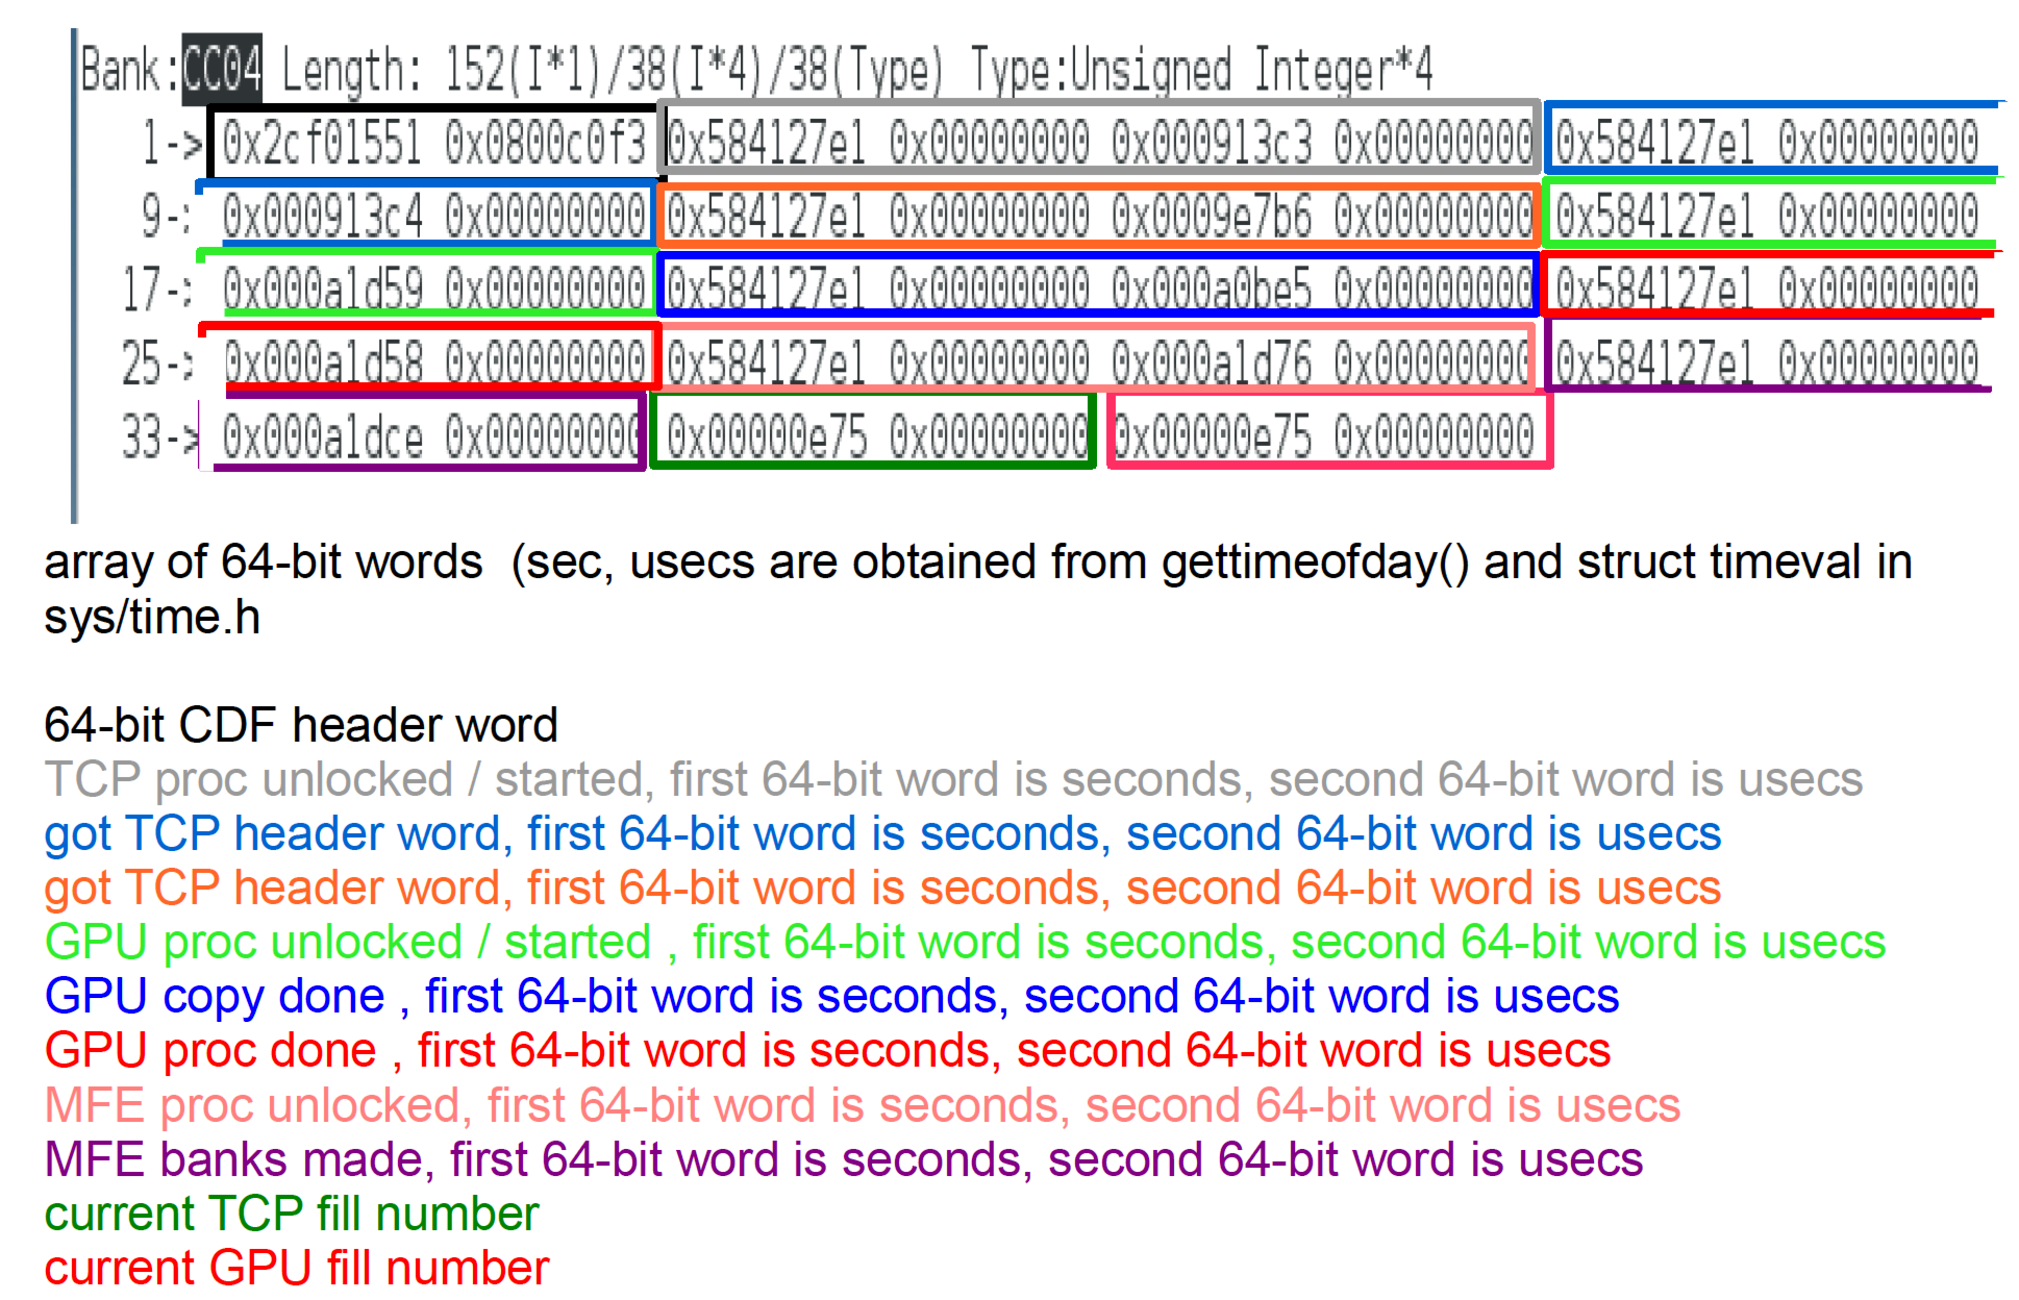
\includegraphics[width=0.85\textwidth]{pics/CCBankFormat.pdf} 
\caption{Data structure for the CC bank (calo performance).}\label{fig:CCBankFormat}
\end{figure}

\subsection{Auxiliary detector-related banks}

\subsubsection*{KH and KQ banks}
These two banks have the same format as the CH and CQ banks.

\subsubsection*{KT bank}
This bank has the same format as the CT bank.

\subsection{CCC related banks}

\subsubsection*{TTCA, TTCR, TTCZ banks}

\begin{figure}[htbp]
\centering
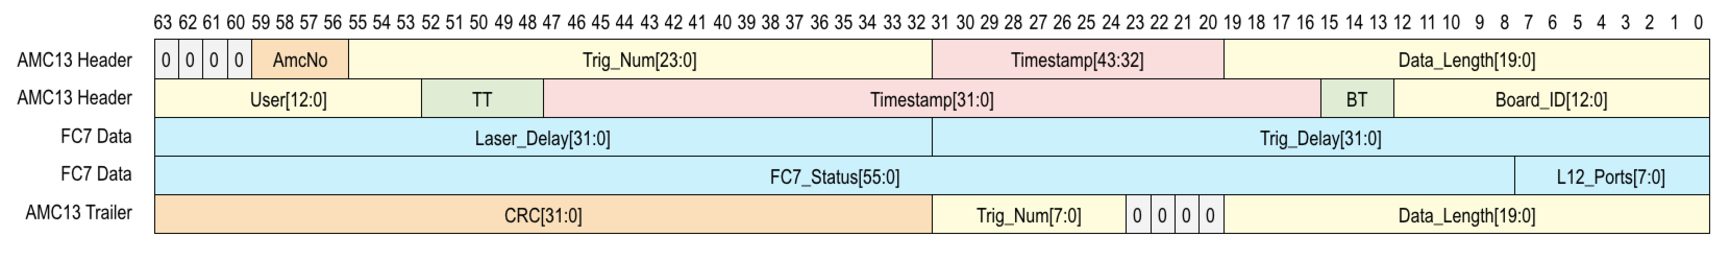
\includegraphics[width=0.85\textwidth]{pics/EncoderFC7.pdf} 
\caption{Data structure for encoder FC7.}\label{fig:EncoderFC7}
\end{figure}

\begin{figure}[htbp]
\centering
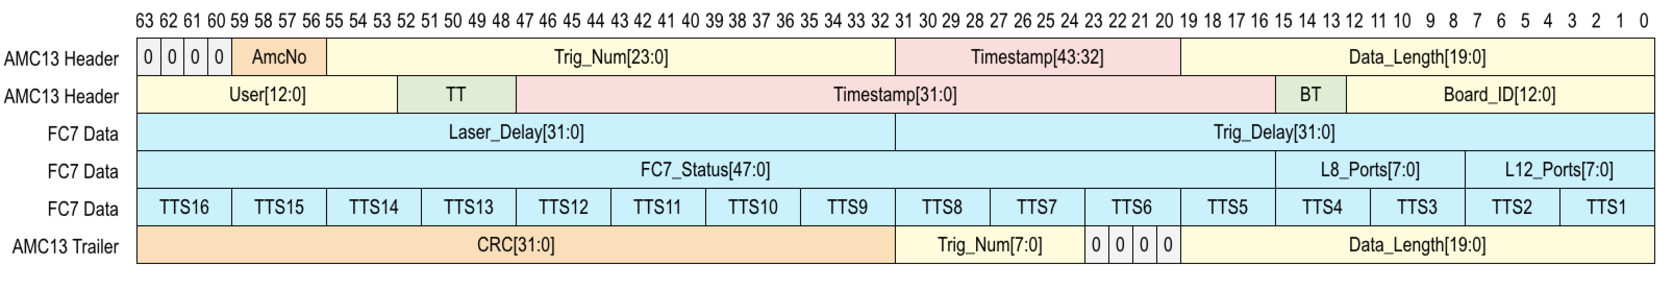
\includegraphics[width=0.85\textwidth]{pics/FanoutFC7.pdf} 
\caption{Data structure for fanout FC7.}\label{fig:FanoutFC7}
\end{figure}


\subsection{Field related banks}

\subsubsection*{FXPR bank}

\begin{table}[htbp]
\centering
\caption{MIDAS bank structure for the FXPR bank.}
\begin{tabular}{|c|c|c|c|p{4cm}|c|}
\hline
start word index & type      & array length       & field name & content                                                          & struct name \\
\hline
0                & Double\_t & num\_ch            & sys\_clock & system clock                                                     & \multirow{12}{*}{fixed\_t}                  \\
\cline{1-5}
4*num\_ch        & Double\_t & num\_ch            & gps\_clock & gps clock                                                        &                             \\
\cline{1-5}
8*num\_ch        & Double\_t & num\_ch            & dev\_clock & device clock                                                     &                             \\
\cline{1-5}
12*num\_ch       & Double\_t & num\_ch            & snr        & signal to noise ratio                                            &                             \\
\cline{1-5}
16*num\_ch       & Double\_t & num\_ch            & len        & length of each wave form                                         &                             \\
\cline{1-5}
20*num\_ch       & Double\_t & num\_ch            & freq       & frequency extracted                                              &                             \\
\cline{1-5}
24*num\_ch       & Double\_t & num\_ch            & ferr       & frequency error                                                  &                             \\
\cline{1-5}
28*num\_ch       & Double\_t & num\_ch            & freq\_zc   & frequency extracted, zero crossing                               &                             \\
\cline{1-5}
32*num\_ch       & Double\_t & num\_ch            & ferr\_zc   & frequency error, zero crossing                                   &                             \\
\cline{1-5}
36*num\_ch       & UShort\_t & num\_ch            & health     & health indicator of probes                                       &                             \\
\cline{1-5}
37*num\_ch       & UShort\_t & num\_ch            & method     & frequency extraction method                                      &                             \\
\cline{1-5}
38*num\_ch       & UShort\_t & num\_ch * rec\_len & trace      & NMR waveforms: Waveform\_Ch1 + Waveform\_Ch2 + … + Waveform\_Ch6 &     \\    
\hline
\end{tabular} 
\label{tab:fxprtable}
\end{table}

\begin{table}[htbp]
\centering
\caption{Hard-coded macros in the FXPR bank.}
\begin{tabular}{|c|c|c|}
\hline
Name in the code	& Name in this doc &	Value \\
\hline
NMR\_NUM\_FIXED\_PROBES & num\_ch & 378 \\
\hline
NMR\_FID\_LENGTH\_RECORD & rec\_len & 10000 \\
\hline
\end{tabular} 
\label{tab:fxprmacro}
\end{table}


\subsubsection*{TLNP bank}

\begin{table}[htbp]
\centering
\caption{MIDAS bank structure for the TLNP bank.}
\begin{tabular}{|c|c|c|c|p{4cm}|c|}
\hline
start word index &	type	& array length	&field name	&content	& struct name \\
\hline
0	& ULong64\_t & 1 & gps\_clock & Time stamp of the first NMR sample	& \multirow{3}{*}{trolley\_nmr\_t}   \\ 
\cline{1-5}
4	&UShort\_t	& 1 & probe\_index	&probe index	 & \\ 
\cline{1-5}
5	&UShort\_t	&1 & length&	length of the NMR waveform	 & \\ 
\hline
6	&Short\_t & nmr\_len &	trace	&Trolley Probe NMR wavefrom	 & \\ 
\hline
\end{tabular} 
\label{tab:tlnp}
\end{table}

\begin{table}[htbp]
\centering
\caption{Hard-coded macros in the TLNP bank.}
\begin{tabular}{|c|c|c|}
\hline
Name in the code	& Name in this doc & Value \\
\hline
TRLY\_NMR\_LENGTH	 & nmr\_len & 24000 \\
\hline
\end{tabular} 
\label{tab:tlnpmacro}
\end{table}


\subsubsection*{TLBC bank}

\begin{table}[htbp]
\centering
\caption{MIDAS bank structure for the TLBC bank.}
\begin{tabular}{|c|c|c|c|p{4cm}|c|}
\hline
start word & index & type & array length & field name	content & struct name \\ 
\hline
0 & ULong64\_t & 1 & gps\_clock & Time stamp of the first barcode sample & \multirow{3}{*}{trolley\_barcode\_t} \\
\cline{1-5}
4 & UShort\_t & 1 & length\_per\_ch & length of the barcode waveform per channel & \\ 
\cline{1-5}	
5 & UShort\_t	& bc\_ch*bc\_len & traces &	Barcode wavefroms: Waveform\_Ch1 + Waveform\_Ch2 + … + Waveform\_Ch6	 &\\
\hline
\end{tabular} 
\label{tab:tlbc}
\end{table}

\section{Parsers for MIDAS bank data}
Muon g-2 offline analysis framework relies on parsers in the gm2parser namespace hosted under repository gm2unpackers to decode the data. To checkout the codes, 

\begin{Verbatim}[frame=single]
git clone ssh://p-gm2dqm@cdcvs.fnal.gov/cvs/projects/gm2unpackers
\end{Verbatim}
%
Alternatively, you can also use 
\begin{Verbatim}[frame=single]
mrb g gm2dqm
\end{Verbatim}
in our g-2 environment.

\end{document}
